
%(BEGIN_QUESTION)
% Copyright 2010, Tony R. Kuphaldt, released under the Creative Commons Attribution License (v 1.0)
% This means you may do almost anything with this work of mine, so long as you give me proper credit

One extremely useful capability of a ``smart'' valve positioner is the ability to measure and plot the relationship between valve stem position and actuator air pressure.  An example {\it valve signature} is shown here:

$$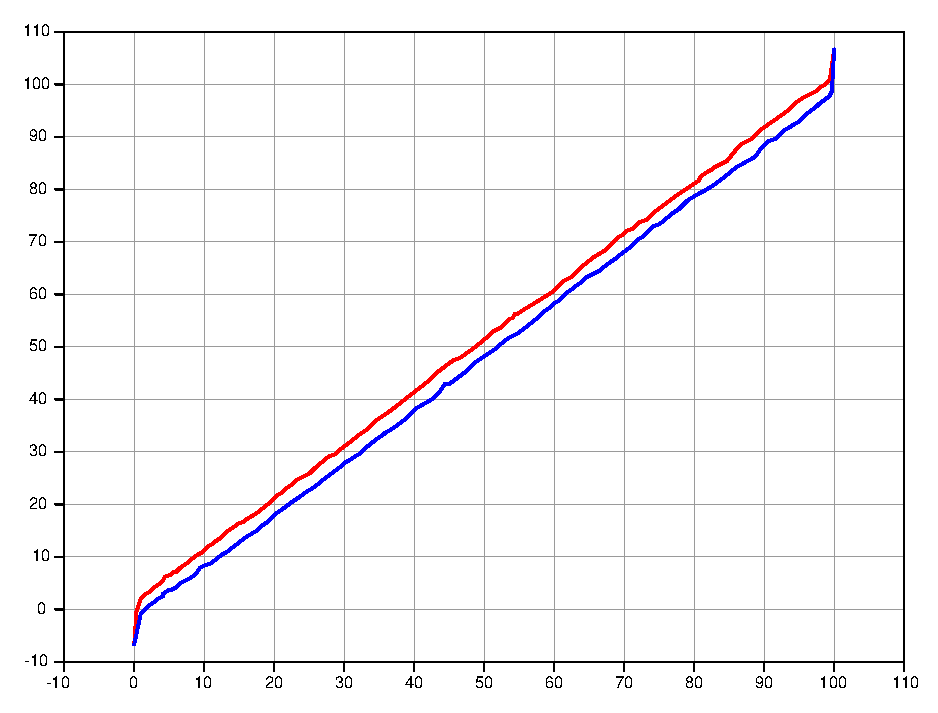
\includegraphics[width=15.5cm]{i04185x01.eps}$$

Closely examine this graph of stem position vs. actuator pressure, and answer the following questions:

\begin{itemize}
\item{} Is this an air-to-open valve, or an air-to-close valve? 
\vskip 10pt
\item{} Which axis of the graph (horizontal or vertical) represents (percent of) valve stem position?  How can you tell?
\vskip 10pt
\item{} Which axis of the graph (horizontal or vertical) represents (percent of) actuator air pressure?  How can you tell?
\vskip 10pt
\item{} What principle of physics makes the plots (approximately) linear throughout the bulk of the travel range?
\vskip 10pt
\item{} Which of the two traces plots the valve while it is {\it opening}?
\vskip 10pt
\item{} Which of the two traces plots the valve while it is {\it closing}?
\vskip 10pt
\item{} What phenomenon accounts for the separation between the two traces?
\end{itemize}

\underbar{file i04185}
%(END_QUESTION)




%(BEGIN_ANSWER)

\noindent
{\bf Partial answer:}

\begin{itemize}
\item{} Is this an air-to-open valve, or an air-to-close valve? {\it It is air-to-open.  We know this from the positive slope of the traces: more air pressure is required to move the valve stem further open.}
\vskip 10pt
\item{} What principle of physics makes the plots (approximately) linear throughout the bulk of the travel range? {\it Hooke's Law describes the linear relationship between force applied to a spring and that spring's displacement:} $F = kx$
\vskip 10pt
\item{} What phenomenon accounts for the separation between the two traces?  {\it Packing friction!}
\end{itemize}

%(END_ANSWER)





%(BEGIN_NOTES)

\begin{itemize}
\item{} Is this an air-to-open valve, or an air-to-close valve? {\it It is air-to-open.  We know this from the positive slope of the traces: more air pressure is required to move the valve stem further open.}
\vskip 10pt
\item{} Which axis of the graph (horizontal or vertical) represents (percent of) valve stem position? {\it The horizontal axis.  We can tell this by the steep ``down'' and ``up'' turns at each end of the plots: here actuator pressure spikes with little or no motion of the stem because the stem has reached its mechanical limit.}
\vskip 10pt
\item{} Which axis of the graph (horizontal or vertical) represents (percent of) actuator air pressure? {\it The vertical axis, for the same reason as above.}
\vskip 10pt
\item{} What principle of physics makes the plots (approximately) linear throughout the bulk of the travel range? {\it Hooke's Law describes the linear relationship between force applied to a spring and that spring's displacement:} $F = kx$
\vskip 10pt
\item{} Which of the two traces plots the valve while it is {\it opening}?  {\it The upper trace shows the valve when it is opening.  We know this because more air pressure is required to lift the stem further against the force of packing friction.}
\vskip 10pt
\item{} Which of the two traces plots the valve while it is {\it closing}?  {\it The lower trace shows the valve when it is closing.  We know this because less air pressure is required to allow the spring's natural restorative force to overcome the force of packing friction.}
\vskip 10pt
\item{} What phenomenon accounts for the separation between the two traces?  {\it Packing friction!}
\end{itemize}









\filbreak \vskip 20pt \vbox{\hrule \hbox{\strut \vrule{} {\bf Virtual Troubleshooting} \vrule} \hrule}

\noindent
{\bf Predicting the effect of a given fault:} present each of the following faults to the students, one at a time, having them comment on all the effects each fault would produce.

\begin{itemize}
\item{} Valve spring adjuster loosened
\item{} Valve spring adjuster tightened
\item{} Packing nuts tightened too far
\item{} Worn seat
\item{} Bent valve stem
\item{} Valve stem and actuator stem coupled too far apart
\item{} Missing actuator spring
\item{} Chunk of metal stuck between the plug and the seat
\item{} I/P calibration zero error (positive error ; too much P for I)
\item{} Valve and actuator stems uncouple ; positioner reading valve stem position
\item{} Valve and actuator stems uncouple ; positioner actuator valve stem position
\end{itemize}


%INDEX% Final Control Elements, valve: diagnostic signature for pneumatic actuator

%(END_NOTES)


